% +---------------------------------------------------------------+
% | Author :    Noémie Plancherel, HEIG-VD
% | Date :      18.04.2022
% +---------------------------------------------------------------+

\chapter{Étude sécuritaire}
\label{ch:etude_secu}

Ce chapitre est dédié à toute l'analyse sécuritaire des gestionnaires de mots de passes en général. Nous allons dans un premier temps décrire comment ces applications sont sécurisées en fonction de leur type, puis présenter les différents algorithmes utilisés dans les candidats sélectionnés

\section{Implémentation de la sécurité dans les gestionnaires de mots de passe}

Dans cette section, afin de se baser sur des gestionnaires de mots de passe déjà existants et de pouvoir comparer les différentes sécurités implémentées, nous allons reprendre les 9 candidats sélectionnés dans la partie \hyperref[ch:etude_marche]{\textit{étude de marché}}, c'est-à-dire; \textit{LastPass}, \textit{Dashlane}, \textit{1Password}, \textit{KeePass}, \textit{Bitwarden}, \textit{NordPass}, \textit{Padloc}, \textit{Keeper} et \textit{Firefox}. Toutes les informations citées sont basées sur les \textit{security whitepapers} des constructeurs\cite{lastpasssecurity}\cite{dashlanesecurity}\cite{1passwordsecurity}\cite{keepasssecurity}\cite{bitwardensecurity}\cite{padlocsecurity}\cite{keepersecurity}\cite{nordpasssecurity}.

Les gestionnaires de mots de passe sélectionnés ont un fonctionnement plutôt similaire, au final cette méthode est plutôt classique dans les architectures des applications. Un \textit{master password} (qui est seulement connu par l'utilisateur) est généré ou entré par l'utilisateur et va permettre le déverrouillage de l'application et le chiffrement / déchiffrement en local de toutes les données stockées. 

À part pour les gestionnaires en local qui gèrent la sécurité différemment, les gestionnaires qui utilisent la synchronisation avec le cloud mettent en avant le \textit{Zero-knowledge encryption}. C'est une méthode qui va permettre un chiffrement \textit{end-to-end} et qui va sécuriser au mieux les données personnelles et sensibles des utilisateurs, des serveurs du constructeur. En sachant que toutes les données sont stockées dans le cloud du provider, afin d'éviter que n'importe qui puisse y avoir accès, toutes les données sont chiffrées avant d'être envoyées au serveur. Ainsi, les données sont uniquement déchiffrées sur le device de l'utilisateur et la clé de chiffrement reste également en local.

Nous allons décrire dans les sous-sections suivantes comment la sécurité est implémentée dans les gestionnaires de mots de passe en fonction de leur type afin d'aller un peu plus en détail. Nous nous concentrons sur 3 types différents de gestionnaires de mots de passe:

\begin{enumerate}
	\item \textbf{Browser-based}, qui sont des gestionnaires de mots de passe directement intégré dans le navigateur (Google Chrome, Firefox, etc.)
	\item \textbf{Cloud/local-based}, qui fonctionnent en local et avec le cloud et peuvent être multi-plateformes. Ce sont des applications tierces.
	\item \textbf{Local-based}, qui fonctionnent uniquement en local et qui n'ont aucune donnée synchronisée entre plusieurs devices. 
\end{enumerate}

\subsection{Les gestionnaires browser-based}
Les gestionnaires de mots de passe \textit{browser-based} proposent des fonctionnalités classiques et ne sont pas très poussés. Ce sont des applications légères qui sont pensées pour faciliter au mieux les internautes.\cite{Browser}

Par défaut, ces applications n'activent pas de \textit{master password} et certaines n'en proposent même pas pour ajouter un chiffrement supplémentaire. Toutefois, ils proposent la fonctionnalité de 2FA. Afin d'illustrer au mieux nos propos, nous allons nous baser sur le gestionnaire intégré Firefox.

\textbf{Firefox} fonctionne localement ou avec la synchronisation qui demande l'utilisation du cloud. Si la synchronisation n'est pas activée, les mots de passes stockés sont directement chiffrés sur l'appareil et sont ajoutés à un fichier \textit{logins.json} qui se trouve dans le répertoire de l'utilisateur. 

Il propose également la fonctionnalité d'ajouter un master password afin d'avoir une couche sécuritaire supplémentaire (par défaut, cette fonction est désactivée), ainsi, sans un mot de passe principal et sans l'activation du 2FA, les mots de passe sont accessibles en clair sur le navigateur dès le moment où on a accès à l'appareil et que l'utilisateur est connecté à son compte (ce qui est fortement probable, car le compte reste connecté, même après une fin de session). Toutefois, lors de l'ajout d'un master password, ce dernier est uniquement défini en local et n'est pas synchronisé entre profils ou appareils, mais il chiffrera toutes les données en local. 

Au niveau du fonctionnement\cite{firefoxEncr} (sans master password), les identifiants sont chiffrés à l'aide de 3DES-CBC et sont directement stockés dans un fichier JSON \textit{logins.json} encodés en ASN.1 puis en Base64. La clé de chiffrement est stockée dans une base de donnée \textit{key4.db}. Il existe actuellement des outils pour déchiffrer les mots de passe du gestionnaire.

Nous allons illustrer ci-dessous, comment se passe le déchiffrement d'un mot de passe d'une entrée stockée en local dans les gestionnaire de mots de passe Firefox. La référence de ce schéma est un GitHub\cite{firepwd} qui explique comment sont protégés les mots de passe.

\begin{figure}[H]
	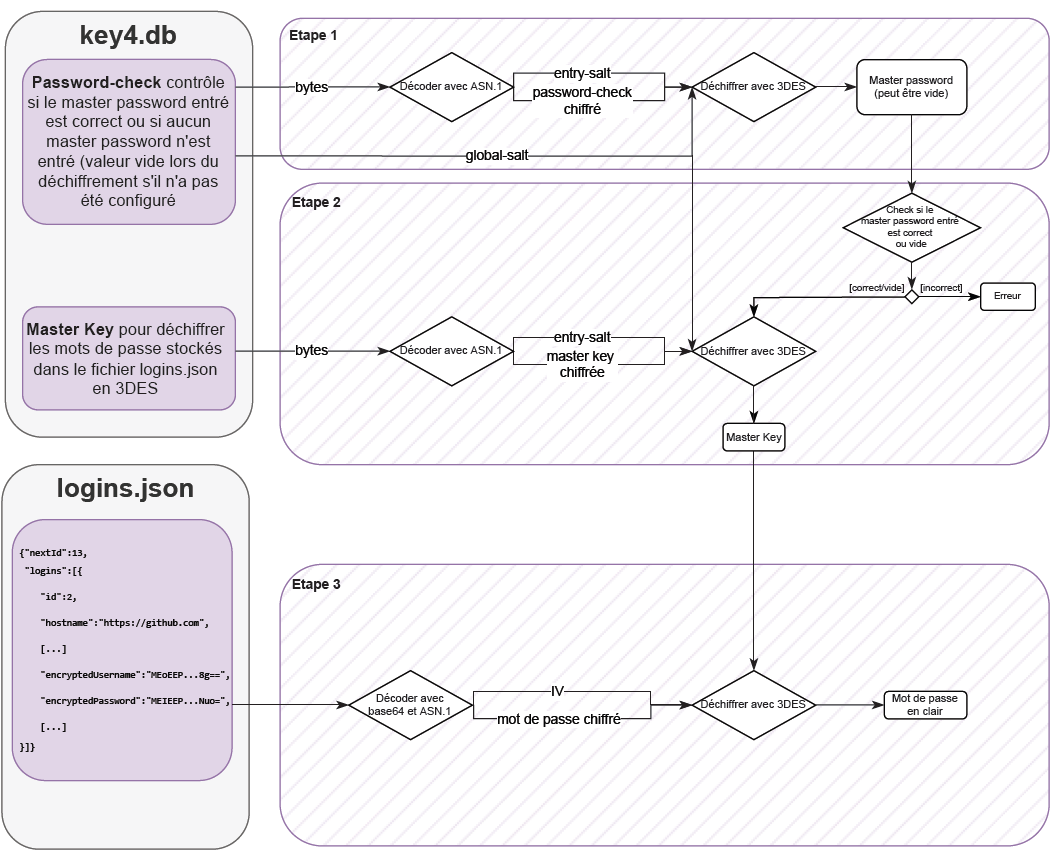
\includegraphics[width=15.5cm]{images/firefox_local.png}
	\centering
	\caption{Déchiffrement d'un mot de passe en local sur Firefox}
\end{figure}

Si l'option de synchronisation (\textit{Firefox Sync}) est activée\cite{firefoxsync}, les données stockées sur les serveurs Mozilla seront chiffrées. Nous pouvons se baser sur le schéma suivant qui explique le processus de synchronisation des données avec les serveurs Mozilla:
\begin{figure}[H]
	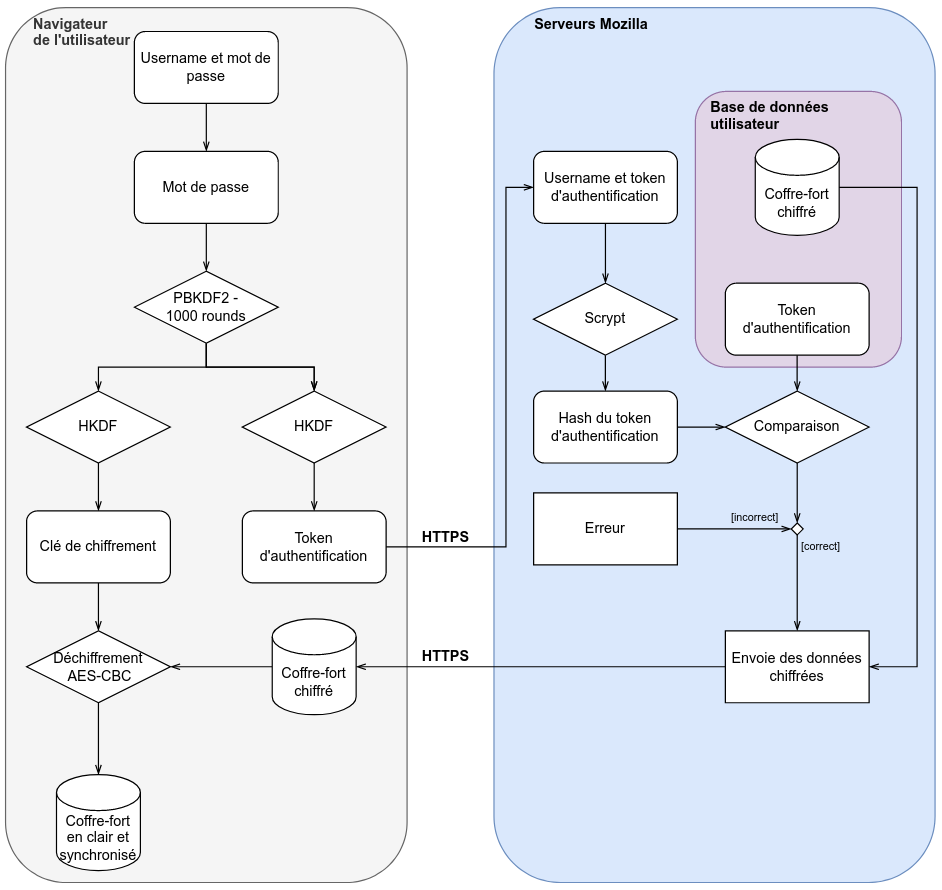
\includegraphics[width=15.5cm]{images/firefox_sync.png}
		\centering
	\caption{Schéma de synchronisation de données sur Firefox}
\end{figure}

Les données chiffrées sont protégées avec HMAC-SHA256 afin de pouvoir authentifier les données avant de les déchiffrer. La méthode utilisée est Encrypt-then-MAC. Cela permet de protéger l'intégrité de toutes les données chiffrées.

Comme cité précédemment, lors d'un ajout de master password afin de protéger les données localement, Firefox va tout d'abord chiffrer les données localement (le stockage se fait comme expliqué plus haut) et va les re-chiffrer lors de la synchronisation avec le processus expliqué à l'aide du schéma.

Lorsque les serveurs Mozilla envoient les données à l'utilisateur pour la synchronisation, il envoie toutes les données stockées (tous les identifiants enregistrés),  même si qu'une modification n'a été effectuée.

Au final, ce design cryptographique est plutôt classique au sein des gestionnaires de mots de passe qui utilisent les serveurs du constructeur pour stocker les données.

Les autres gestionnaires de mots de passe browser-based fonctionnent en général de la même manière avec les données synchronisées. Chrome stocke également les identifiants dans un fichier local protégé avec DPAPI (Microsoft's Data Protection API).
\subsection{Les gestionnaires local-based}
\label{local}
Pour les gestionnaires qui fonctionnent uniquement en local, nous allons nous baser sur l'implémentation sécuritaire de \textbf{KeePass}, qui est open-source, ce qui peut faciliter à comprendre tout le concept. Dans cette section, nous n'allons pas détailler toute l'architecture mais rester plutôt en surface. D'autres gestionnaires de mots de passe fonctionnent également en \textit{offline} avec un stockage local, cependant lors de la première connexion, il y a quand même des informations envoyées aux serveurs du constructeur (comme 1Password par exemple), ce qui n'est pas le cas pour l'application de base KeePass.

Etant donné que KeePass ne fonctionne qu'en local, il est important de bien gérer la mémoire et le stockage de données sensibles.

Toutes les données se trouvent dans un fichier de base de données spécial \textit{.kdbx}. Ce fichier contient toutes les données du gestionnaire (mots de passe, usernames, etc.) et est chiffré (également compressé en GZIP si on le souhaite). Dans la version de KeePass 2.x, les chiffrements supportés sont AES256-CBC et ChaCha20. 

La base de données est stockée où l'utilisateur le souhaite (avec une possibilité de la stocker dans un cloud), c'est pourquoi la sécurité repose sur la complexité du mot de passe. Elle est structurée avec un header et un contenu\cite{keepassstruct}\cite{keepassieee}.

Dans le header, sont stockées différentes informations; un UUID indiquant le cipher, une indication si le fichier est compressé, différentes seed (voir \ref{schema_keepass}), l'IV pour le chiffrement et des bytes pour l'authentification (générés aléatoirement lors de la sauvegarde de la base de données). Le corps du fichier contient des blocs hachés avec HMAC-SHA256 et des blocs de données qui ont un format XML lorsqu'ils sont déchiffrés.

Afin d'expliquer au mieux la structure de la base de données, nous avons établi un schéma qui présente tous les champs du header et du contenu de la base de données.

\begin{figure}[H]
	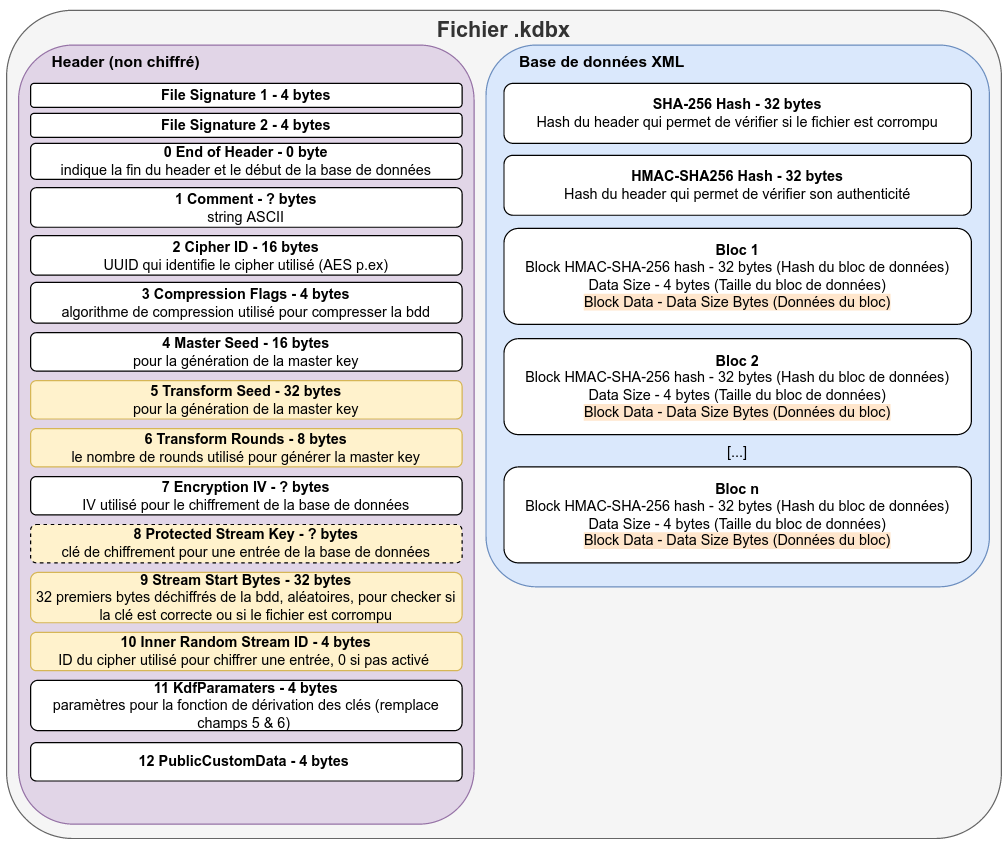
\includegraphics[width=15.5cm]{images/keepass_local.png}
	\centering
	\caption{Contenu du fichier .kdbx de KeePass}
	\label{kp_file}
\end{figure}

Nous avons représenté la structure de la version 4 du fichier \textit{.kdbx}\cite{kp4}. Le header contient des champs qui ne sont pas forcément présents dans chaque fichier (en traitillé sur le schéma). Ces derniers apparaissent si on souhaite effectuer un double chiffrement et chiffrer en plus chaque entrée de la base de données (chaque mot de passe stocké). De plus, les champs en jaune permettent la comptabilité entre la version 3.1 et 4 des fichiers \textit{.kdbx}, cependant ils ne sont plus utilisés dans la version récente. 

La partie données du fichier contient deux champs hashés afin de vérifier l'authenticité du header. Ces champs ne sont pas chiffrés afin qu'on ne doive pas déchiffrer toutes les données pour vérifier que le master password entré est correct. Toutes les données sont séparées en blocs de données et chaque bloc possède un hash (non-chiffré) afin de contrôler l'authenticité du bloc. Le schéma \textit{Encrypt-Then-Mac} est utilisé, c'est-à-dire que le hash est généré à l'aide de données chiffrées, qui sont surlignées en orange sur le schéma ci-dessus. 

Au niveau de l'utilisation de la mémoire du processus, lorsqu'il y a une interaction avec une entrée de la base de données, elle est chargée en mémoire. La protection de la mémoire s'applique uniquement aux données sensibles telles que la Master key et des mots de passe, le username ou les notes. Pour certaines opérations, comme la copie dans le presse-papier ou l'affichage des données en clair, KeePass doit rendre les données sensibles disponibles de manière non chiffrée dans la mémoire du processus pendant un court instant.  

Dès le moment où l'application est verrouillée ou le processus arrêté, la mémoire est nettoyée afin qu'elle ne contienne aucune information sensible.

 \newpage

\begin{wrapfigure}[28]{l}{0.55\textwidth} 
	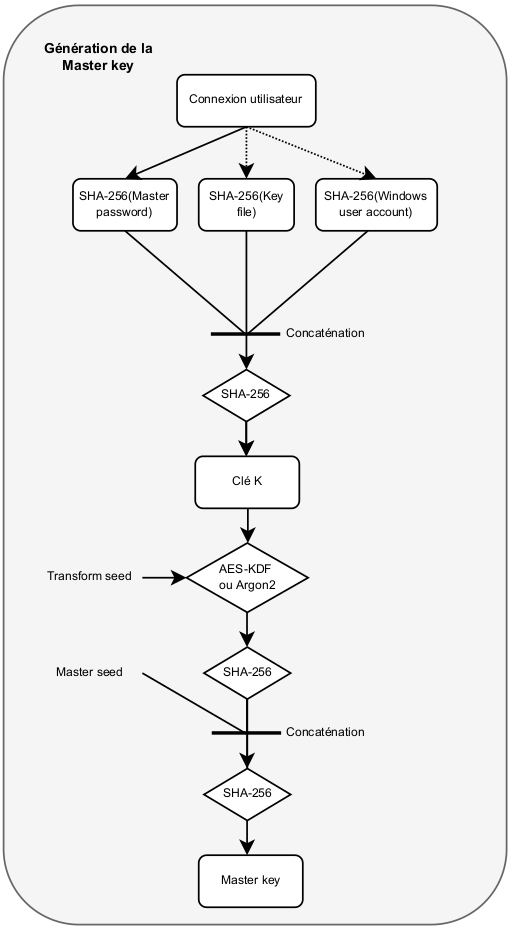
\includegraphics[width=0.5\textwidth]{images/keepass_generation_key.png}
	\caption{Génération de la Master key sur Keepass \label{schema_keepass}}
\end{wrapfigure}

La Master key sur KeePass prend plusieurs arguments différents et est générée d'une manière assez complexe. L'utilisateur doit obligatoirement fournir un master password, et peut également utiliser un key file et / ou le compte utilisateur Windows. 

Chaque composant est haché avec SHA-256 et sont concaténés et hachés ensemble. En sortie, on a une clé composite K qui va être dérivée à l'aide de AES-KDF ou Argon2. Les paramètres de ces deux algorithmes peuvent être configurés dans les paramètres de la base de données.

Chaque sortie est hachée avec SHA-256 et au final, on obtient la Master key qui permettra de déchiffrer la base de données.

Les deux différentes seeds utilisées dans la génération de la clé sont stockées dans le header de la base de données \textit{.kdbx}.

Cette architecture permet de se protéger contre les attaques par dictionnaires et le brute-force de la Master key.
\newline\newline\newline\newline\newline
\subsection{Les gestionnaires cloud/local-based}
\label{lp}
Les gestionnaires de mots de passes cloud/local-based ont tous une architecture similaire dû au fait que toutes les données sont stockées sur les serveurs du constructeur. Il y a des différences avec l'authentification de l'utilisateur et des algorithmes cryptographiques choisis, mais le design sécuritaire a la même base au niveau de la connexion de l'utilisateur et du chiffrement du gestionnaire. 

Ainsi, afin d'expliquer un peu plus en détail le fonctionnement d'un gestionnaire cloud-based, nous allons prendre l'exemple de \textbf{LastPass}. Nous allons nous baser sur le schéma ci-dessous afin d'appuyer nos propos.
\begin{figure}[h!]
	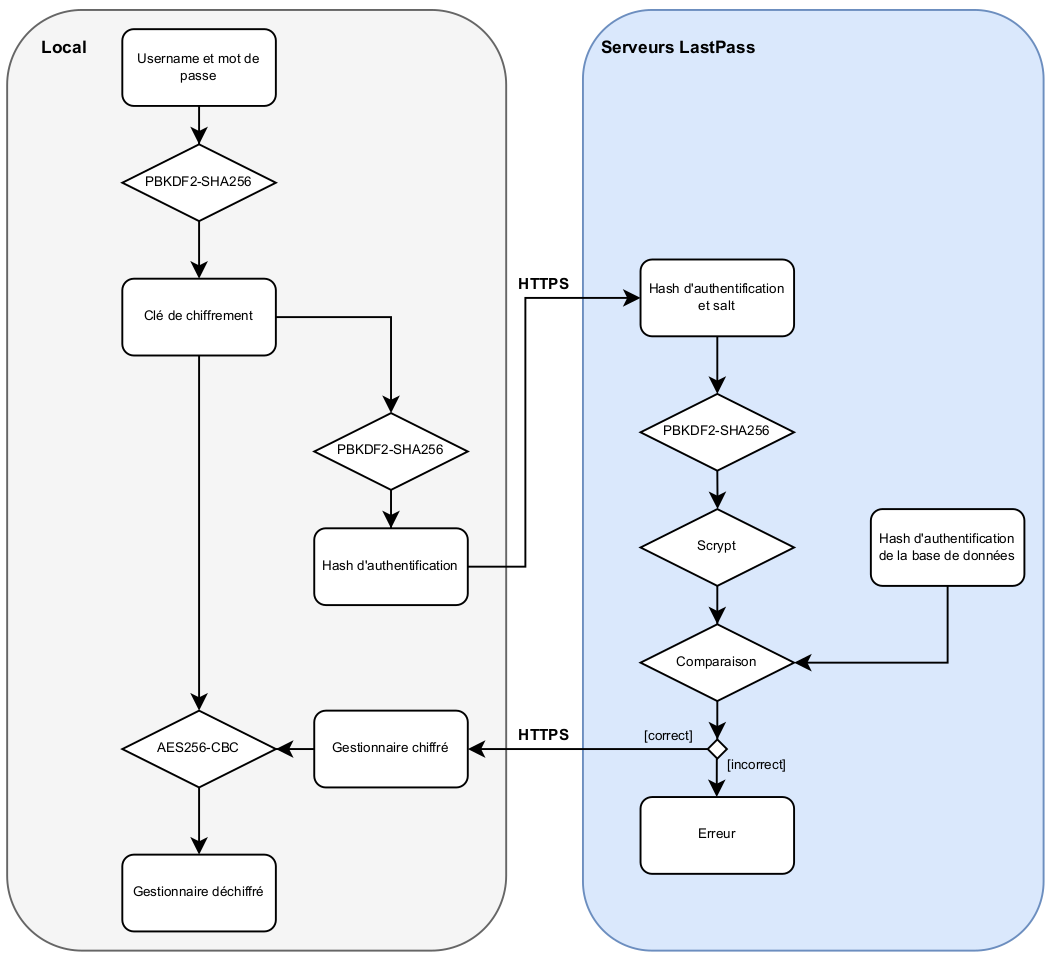
\includegraphics[width=15.5cm]{images/lastpass_encr.png}
	\centering
	\caption{Schéma de déchiffrement de LastPass}
\end{figure}

Afin de générer la clé de chiffrement, ce dernier dérive le master password en utilisant le nom d'utilisateur comme sel. Il utilise l'algorithme PBKDF2-SHA256 avec 100'100 rounds. Du côté client, la sortie est hashée une fois de plus et est envoyée aux serveurs du provider afin de comparer ce hash d'authentification à celui qui est dans la base de données.

Toutes les données de l'utilisateur sont chiffrées avec AES-256-CBC avec la clé de chiffrement générée depuis le master password.

Les serveurs de LastPass stockeront la hash d'authentification et le coffre-fort de l'utilisateur chiffré. La clé de chiffrement reste sur le device en local dans la mémoire du processus.

Tous les gestionnaires de mots de passe incluent la fonctionnalité de 2FA (voire MFA). La façon dont est géré cette sécurité additionnelle dépend du constructeur et de la méthode utilisée, certains stockent une clé supplémentaire sur les serveurs, d'autres stockent en local les informations (notammant avec les facteurs biométriques). Lors de la génération de la clé de chiffrement, le master password et les facteurs supplémentaires sont combinés pour y dériver la clé.
\section{Partage d'informations}
La majorité des gestionnaires de mots de passe proposent le partage d'informations entre plusieurs utilisateurs. Nous n'allons pas entrer dans tous les détails dans cette sous-section afin de rester bref et d'expliquer le schéma général du partage de données.

Pour cette fonctionnalité, nous utilisons la cryptographie asymétrique avec RSA. Dès l'inscription et la création du coffre-fort de l'utilisateur, une paire de clés de 2048 bits [publique, privée] est générée. 

La façon dont est géré le stockage des clés dépend du constructeur mais en général, la clé publique est envoyée aux serveurs, tandis que la clé privée est soit stockée avec les données personnelles de l'utilisateur, soit envoyée aux serveurs. Cette dernière (privée au serveur) est chiffrée afin de garantir sa protection et étant donné qu'elle est personnelle et n'est pas censé être transmise entre utilisateurs, cela est tout à fait concevable. Pour le chiffrement, soit la même clé pour le chiffrement des données est utilisée ou une clé symétrique supplémentaire est générée. 

Afin d'illustrer concrètement le processus complet de partage, nous allons nous baser sur le gestionnaire \textbf{Dashlane} et nous montrerons un exemple où Alice souhaiterait partager un identifiant à un autre utilisateur, Bob.
\newpage 
\begin{figure}[h!]
	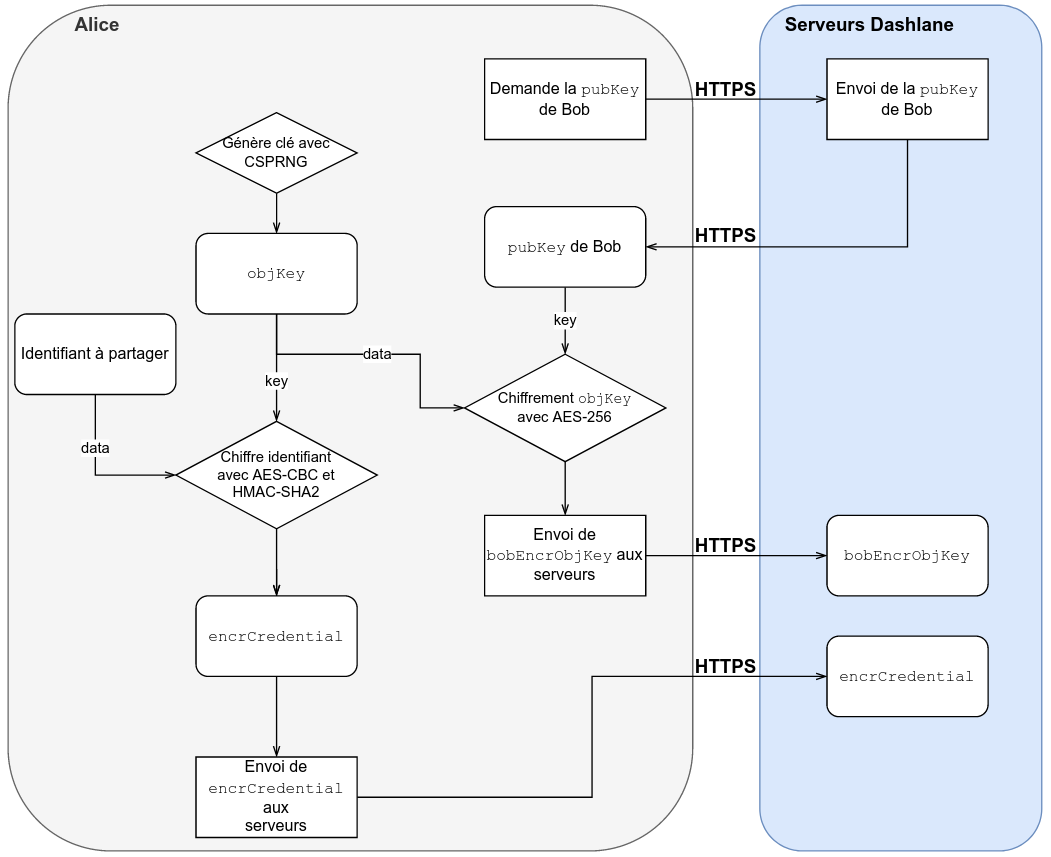
\includegraphics[width=15.5cm]{images/dashlane_share_alice.png}
	\centering
	\caption{Partage d'un identifiant sur Dashlane}
\end{figure}

Les différents éléments à considérer:
\begin{itemize}
	\item \verb|pubKey| est la clé publique de Bob et va servir à chiffrer l'information à partager
	\item \verb|privKey| est la clé privée de Bob
	\item \verb|objKey| est la clé symétrique AES-256 générée avec un CSPRNG\footnote{\textit{Cryptographically secure pseudorandom number generator approprié pour la cryptographie} est un générateur de nombre pseudo-aléatoire} qui chiffre l'identifiant à partager
	\item \verb|bobEncrObjKey| est la clé unique de l'objet chiffrée avec la clé publique de Bob
	\item \verb|encrCredential| est l'identifiant à partager chiffré avec la clé générée à l'étape précédente
\end{itemize}

A chaque fois qu'un élément doit être partagé, on génère une clé symétrique aléatoirement qui est stockée sur les serveurs du provider à l'aide de la clé publique de l'utilisateur concerné. La clé est générée à l'aide d'un CSPRNG. Elle va permettre de chiffrer les identifiants avec AES-CBC et HMAC-SHA2, qui va permettre de garantir la confidentialité ainsi que l'intégrité en l'authentifiant.
\begin{figure}[h!]
	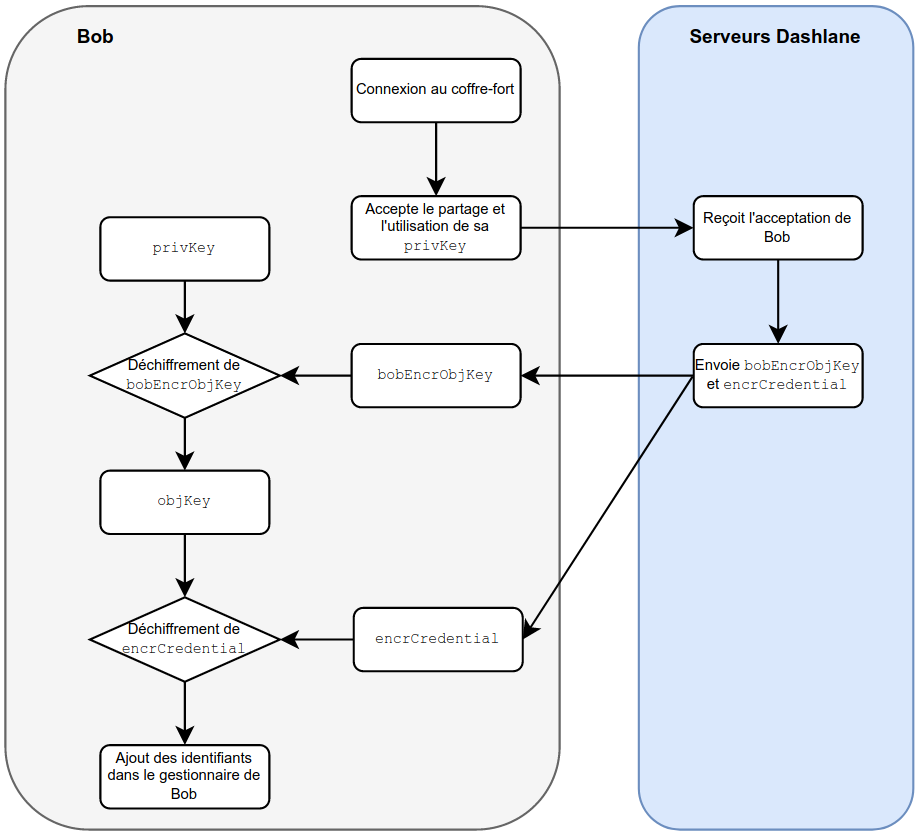
\includegraphics[width=15.5cm]{images/dashlane_share_bob.png}
	\centering
	\caption{Réception d'un partage d'identifiant sur Dashlane}
\end{figure}

Afin de récupérer le partage, Dashlane demande à l'utilisateur d'accepter l'envoi d'Alice pour qu'il accepte d'utiliser sa clé privée. Tout dépend de l'architecture de l'application, mais cette dernière doit d'abord être déchiffrée avant d'être utilisée pour déchiffrer l'identifiant envoyé par Alice. 

Les identifiants partagés sont ajoutés finalement au coffre-fort de Bob. Ces derniers seront synchronisés par la suite sur tous les autres appareils de Bob dès qu'il sera connecté dessus. 

Certains gestionnaires proposent de faire des dossiers partagés. Dans le cadre d'entreprises, cela est une fonctionnalité très utile. Le processus est le même que pour le partage avec une personne. Une clé pour le dossier à partager est générée et on chiffre chaque clé publique de tous les utilisateurs concernés à l'aide de cette dernière.

\section{4 états du gestionnaire de mot de passe \label{etats}}
Les gestionnaires de mots de passe ont généralement 4 états différents: \textit{Not Configured}, \textit{Not Running}, \textit{Unlocked State} et \textit{Locked State}. Nous allons expliquer plus en détails comment ils fonctionnent lorsqu'ils sont dans les différents états. Nous nous basons sur un article qui analyse le management des secrets\cite{iseexploit}.

\subsection{État \textit{Not Configured}}
On définit cet état lorsque l'application n'a jamais été utilisée après son installation et n'a pas encore été configurée, c'est-à-dire insciption de l'utilisateur avec la création de son compte. Aucun secret n'est stocké en mémoire.
\subsection{État \textit{Not Running}}
C'est l'état du password manager lorsqu'il n'a pas été lancé depuis le dernier redémarrage du système ou a été arrêté par un utilisateur mais qu'il a déjà été configuré. Dans cet état, le gestionnaire doit garantir qu'il n'y a aucune donnée sensible stockée sur le disque qui permettrait de compromettre le coffre-fort, comme une clé de chiffrement ou le master password.
\subsection{État \textit{Unlocked State}}
Cet état indique que le gestionnaire fonctionne et donc, l'utilisateur a entré son master password afin de déchiffrer toutes les données afin d'avoir accès aux informations stockées. Le gestionnaire doit garantir qu'il n'est pas possible d'extraire d'information sensible de la mémoire. De plus, à part pour les mots de passe avec lesquels l'utilisateur a eu une interaction (affichage, accès ou copie), il ne devrait pas être possible d'extraire déchiffrés depuis la mémoire le reste des mots de passe.
\subsection{État \textit{Locked State}}
Nous considérons cet état lorsque l'utilisateur a lancé le gestionnaire (déjà configuré) sans avoir encore entré le master password, qu'il a lui même verrouillé son gestionnaire ou qu'il y a eu un timeout de session. À ce moment, il ne devrait pas y avoir de données sensibles stockées sur le disque et sur la mémoire RAM afin d'éviter toute extraction. 

Ci-dessous un schéma qui permet de résumer tout ce qui a été expliqué dans les sections précédentes:

\begin{figure}[H]
	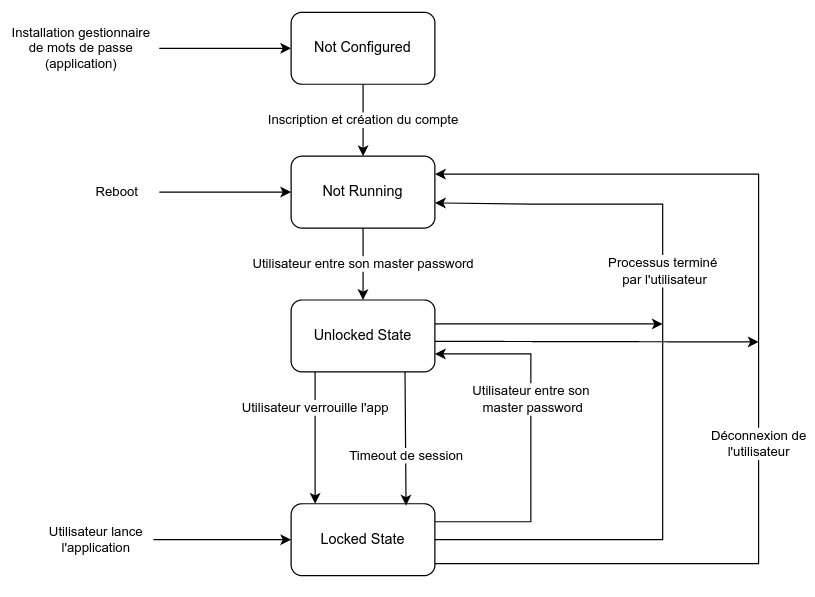
\includegraphics[width=14.5cm]{images/states.png}
	\centering
	\caption{Différents états d'un gestionnaire de mots de passe}
\end{figure}

\section{Algorithmes cryptographiques}
Afin d'avoir une bonne vue d'ensemble de l'architecure sécuritaire des gestionnaires de mots de passe sélectionnés pour notre étude, nous allons résumer les algorithmes cryptographiques utilisés pour le chiffrement des données, la dérivation des clés et l'authentification.

{\small
\begin{longtable}[c]{|l|c|cc|c|}
				\hline
				& Chiffrement des données & \multicolumn{2}{c|}{Dérivation des clés}    & Partage de données                                                                                                                      \\ \hline
				LastPass  & AES-CBC 256             & \multicolumn{2}{c|}{\begin{tabular}[c]{@{}l@{}}PBKDF2-SHA2\\ 100'000 rounds\end{tabular}}     & RSA-2048   \\ \hline
				Dashlane  & AES-256                 & \multicolumn{1}{c|}{Argon2d} & \begin{tabular}[c]{@{}l@{}}PBKDF2-SHA2\\ 200'000 rounds\end{tabular} & RSA-2048  \\  \hline
				1Password & AES-GCM 256             & \multicolumn{2}{c|}{\begin{tabular}[c]{@{}l@{}}PBKDF2-SHA2\\ 100'000 rounds\end{tabular}} & RSA-OAEP 2048      \\  \hline
				KeePass   & AES-CBC 256/ChaCha20 & \multicolumn{1}{c|}{AES-KDF} & Argon2   & -                                                             \\  \hline
				Bitwarden & AES-CBC 256             & \multicolumn{2}{c|}{\begin{tabular}[c]{@{}l@{}}PBKDF2-SHA2\\ 100'000 rounds\end{tabular}}     & RSA-2048     \\  \hline
				NordPass  & XChaCha20-Poly1305-IETF               & \multicolumn{2}{c|}{Argon2id}                                                                    &   ?\footnote{Information pas précisée sur leur documentation, toutefois il s'agit sûrement de RSA} \\  \hline
				Padloc    & AES-GCM 256             & \multicolumn{2}{c|}{PBKDF2-SHA2}     & RSA-PSS                                                              \\  \hline
				Keeper    & AES-256                 & \multicolumn{2}{c|}{PBKDF2}         &      RSA                                   \\  \hline
				Firefox   & AES-CBC/3DES-CBC                & \multicolumn{2}{c|}{\begin{tabular}[c]{@{}l@{}}PBKDF2-SHA2 et HKDF\\ 1000 rounds\end{tabular}}                                                              & -    \\ \hline
\caption{Algorithmes cryptographiques des candidats \label{crypto}}
\end{longtable}
}


Nous pouvons remarquer que certains gestionnaire ont plusieurs algorithmes différents pour le même élément, ceci est dû au fait que l'utilisateur a le choix de configurer celui qu'il préfère et que l'application supporte les deux.